% !TEX root = ./../paper.tex

\section{Results}
\label{sec:results}

Artlang as a programming language is a functioning language capable of writing any program.
To validate such a claim, we have written a program in Artlang, an implementation of the Fibonacci sequence.
The language uses FILO (First In Last Out) stacks to store and manipulate data. Each stack is represented by a different shape other than the reserved shapes used by the instructions, and they are initialized on first call.
Stacks can hold an arbitrarily large amount of rational numbers.
Stacks allow the pop, push, move and duplicate operations.
Numbers are defined by their literal counterparts, and the language supports basic arithmetic.
Arithmetic operations are performed by popping the first two elements of the stack, performing the operation, and pushing the result back into the stack.
Artlang allows for flow control through the use of loops, conditional blocks and jump blocks.
Loops are physically represented by a literal loop of connected blocks.
Conditional statements are represented by a question block using a value as a parameter. Positive values are considered true and evaluate the following block, and negative values are considered false and do not evaluate the affected block.


Artlang is based on the physical blocks. Blocks as three-dimensional objects are unwieldy to be described in text.
Therefore, we will use a simplified notation to represent the blocks in planar space.
Every block is represented as a square with the shape of each block inside the square. 
The connections between blocks are represented by arrows between the squares.

\begin{figure}[H]
    \centering
    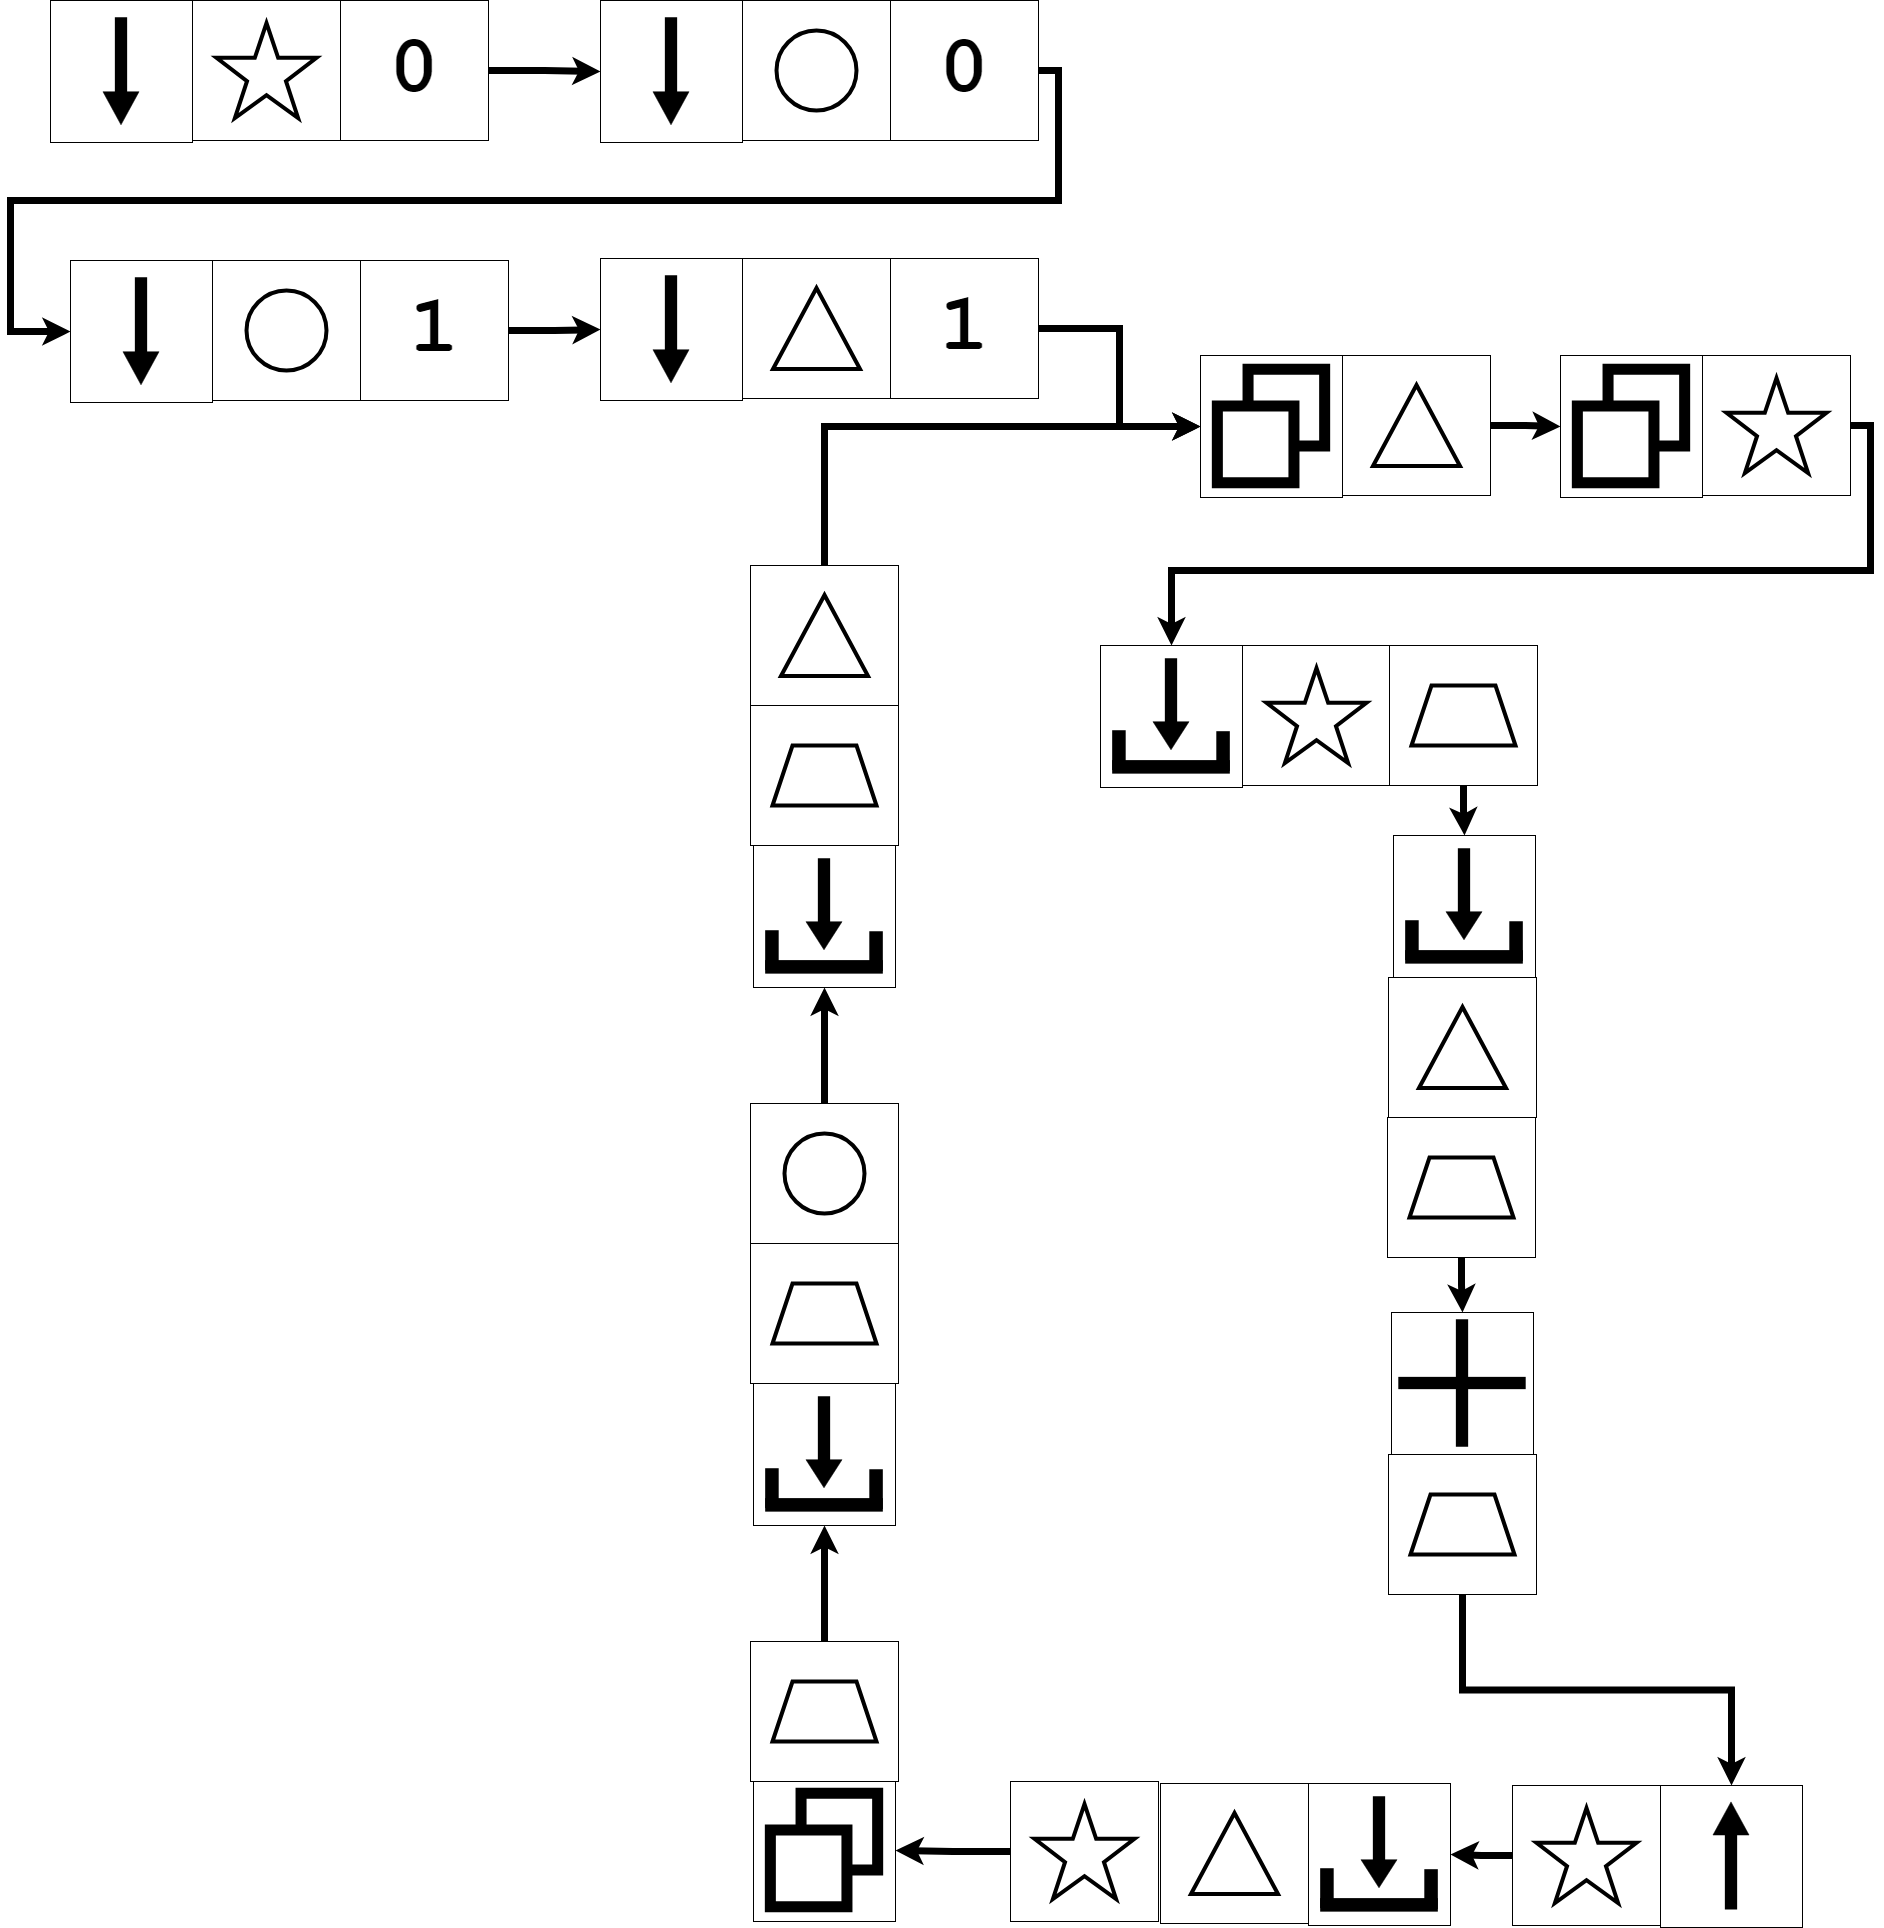
\includegraphics[width=0.5\textwidth]{figures/ArtlangFibpng}
    \caption{Artlang Fibonacci program}
    \vspace{5pt}
    \label{fig:artlangfib}
\end{figure}

The program in Figure \ref{fig:artlangfib} fills the cirle stack with the numbers of the Fibonacci sequence.
It can be rewritten as a more traditional algorithm as follows.

\begin{algorithm}[]
    \caption{Fibonacci sequence in Artlang}
    \begin{algorithmic}
    \State $Push~0~into$ \textbf{Star}
    \State $Push~0~into$ \textbf{Circle}
    \State $Push~1~into$ \textbf{Circle}
    \State $Push~1~into$ \textbf{Triangle}
    \While{True}
        \State $Duplicate$ \textbf{Triangle}
        \State $Duplicate$ \textbf{Star}
        \State $Move$ \textbf{Star} $to$ \textbf{Trapezoid}
        \State $Move$ \textbf{Triangle} $to$ \textbf{Trapezoid}
        \State $Add$ \textbf{Trapezoid}
        \State $Pop$ \textbf{Star}
        \State $Move$ \textbf{Triangle} $to$ \textbf{Star}
        \State $Duplicate$ \textbf{Trapezoid}
        \State $Move$ \textbf{Trapezoid} $to$ \textbf{Circle}
        \State $Move$ \textbf{Trapezoid} $to$ \textbf{Triangle}
    \EndWhile
    \end{algorithmic}
\end{algorithm}

